\begin{frame}
  \begin{block}{Definições}
    \begin{itemize}
      \pause
      \item \alert{\textit{Markov Decision Process} - MDP}
      \begin{itemize}
        \item Ferramenta matemática utilizada para analizar sistemas
        \alert{reativos} complexos e definir \alert{políticas} que minimizem o
        \alert{custo} operacional
      \end{itemize}
      \pause
      \item \alert{\textit{Continuous Time MDP} - CTMDP}
      \begin{itemize}
        \item MPD onde os eventos ocorrem a tempo contínuo (ou seja, a qualquer
        tempo)
      \end{itemize}
      \pause
      \item \alert{Infinite Horizon Problem}
      \begin{itemize}
        \item Processos que persistem por um longo período de tempo
      \end{itemize}
    \end{itemize}
  \end{block}
  \pause
  Este trabalho implementa um modelo do tipo \textit{\textbf{Infinite Horizon
  CTMDP}}
\end{frame}

\begin{frame}
  \begin{block}{Modelagem de um CTMDP}
    \begin{itemize}
      \pause
      \item \alert{\textit{The state space:}} $S$
      \begin{itemize}
        \item Conjunto de todos os estados possíveis
      \end{itemize}
      \pause
      \item \alert{\textit{Sets of actions:}} $\{ A(s) | s \in S\}$
      \begin{itemize}
        \item Para cada estado, um conjunto de todas as ações possíveis
      \end{itemize}
      \pause
      \item \alert{\textit{A set of costs:}} $\{c(s,a) | s \in S, a \in A(s) \}$
      \begin{itemize}
        \item Custo associado a ação $a$ quando o sistema está no
        estado $s$
      \end{itemize}
      \pause
      \item \alert{\textit{A set of transitions probabilities:}}
      $ \{ p_{sz}(a) | s,z \in S, a \in A(s) \}$
      \begin{itemize}
        \item Probabilidade de, no próximo instante de decisão, o sistema estar
        no estado $z$ dado ter tomado a ação $a$ no instante em que
        encontrava-se no estado $s$
      \end{itemize}
      \pause
      \item \alert{\textit{Expected time until next decision:}}
      $ \{ \pi (s,a) | s \in S, a \in A(s) \}$
      \begin{itemize}
        \item Considerando que a ação $a$ foi escolhida no estado $s$
      \end{itemize}
    \end{itemize}
  \end{block}
  \pause
  A partir destas definições, pode-se calcular um política $R*$ que minimiza a
  média da função custo
\end{frame}

\begin{frame}
  \begin{block}{Transição de estados é uma função dependente do tempo}
    \begin{itemize}
      \item Um evento ocorrem em um instante $t_n$
      \item Depois do evento, o estado do sistema muda e, simultaneamente, uma
      decisão é tomada
      \item Entre os instantes $t_n$ e $t_{n+1}$, o comportamento do sistema
      irá depender de ambos estados e ação em $t_n$
    \end{itemize}
  \end{block}
\end{frame}

\begin{frame}
  \begin{figure}[h]
  	\begin{center}
      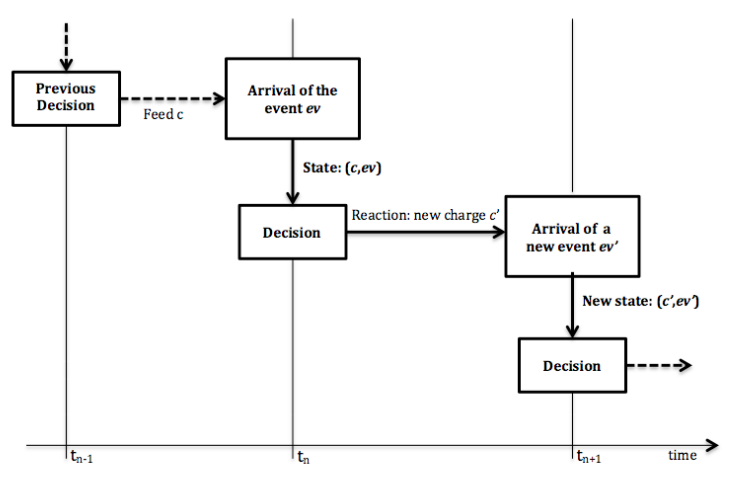
\includegraphics [scale=0.3]{./Figures/StateTransitions}
      \caption {Representação de transição de estados no tempo
      \cite{green-markov}.}
  		\label{fig:arq-imuno}
  	\end{center}
  \end{figure}
\end{frame}

%\begin{frame}
%  \begin{block}{}
%    \begin{itemize}
%      \item
%    \end{itemize}
%  \end{block}
%\end{frame}

%\begin{frame}
%  \begin{block}{}
%  \end{block}
%\end{frame}

%\begin{frame}
%  \begin{figure}[h]
%  	\begin{center}
%      \includegraphics [scale=0.3]{./Figures/Device-Estimates}
%     % \caption {Estimativa de dispositivos conectados à Internet.}
%  		%\label{fig:arq-imuno}
%  	\end{center}
%  \end{figure}
%\end{frame}

%\begin{frame}{Redes de Acesso}
%	\begin{figure}[!htb]
%		\centering
%		\subfloat[DSL]{
%			\includegraphics[height=3.5cm]{./Figures/DSLaccess}
%			\label{figdroopy}}
%		\quad %espaco separador
%		\subfloat[Cable]{
%			\includegraphics[height=3.5cm]{./Figures/CableAccess}
%			\label{figsnoop}}
%		%\caption{Subfiguras}
%		%\label{fig01}
%	\end{figure}
%\end{frame}

%\begin{frame}[fragile]
%\scriptsize
%\begin{verbatim}
%\end{verbatim}
%\end{frame}
